\scanpage{119}
autom de $\unsure{\mathcal T|\mathscr T|\tau}_\gamma$ induisant l'identité sur \inserted{$\simeq$} $\mathcal T_\beta$ plongé, d'où

\[ N_\gamma=N_\beta\,N_{\beta\gamma} \]

Donc il suffit de déterminer les \deleted{\unsure{$N$}} $\unsure{\nu|V}_{\beta-1,\beta,\gamma}$ \inserted{si \deleted{\unsure{$\beta$|$0$}} $1\leq\beta<\gamma$} et $N_{\gamma-1,\gamma}$ pour $\gamma\geq0$

On trouve \deleted{\unsure{c'est}}

\[
\deleted{\unsure{0,1,2|\nu_{0,1,2}}}\quad
\left\{\begin{aligned}
\nu_{-1,0,\gamma}&=2c_\gamma^2\deleted{\unsure{c}}\quad
\begin{cases}\gamma=0&2=\\ \gamma=1&\deleted{\unsure{2c_\gamma^2=}}\ 8=2^3\\
\gamma=2&\deleted{\unsure{2}}\ 32=2^5\end{cases}\\
\nu_{0,1,\gamma}\deleted{\unsure{2}}&=\underset{c_\gamma-1}{\vphantom{\big|}}\!
\begin{cases}\gamma=1&1\\ \gamma=2&3\end{cases}\\
&\deleted{N_{-1,0}=}\\
&\deleted{N_{0,1}=}\qquad\nu_{1,2,\gamma}=c_\gamma-2=2\quad\text{si }\gamma=2\\
&\deleted{N_{1,2}=}
\end{aligned}\right.
\]

\margin{bitriangle du bitriangle \deleted{\unsure{4}}}

\figure{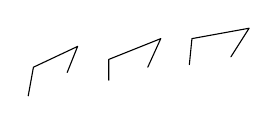
\begin{tikzpicture}[x=0.033cm,y=-0.033cm,line cap=round,line join=round]
\draw (1,19)--(3,8)--(20,0)--(16,10);
\draw (32,13)--(32,5)--(52,-3)--(47,8);
\draw (63,7)--(64,-3)--(86,-7)--(79,4);


\end{tikzpicture}}

$c'_{\beta\gamma}\,(\beta\leq\gamma$

\figure{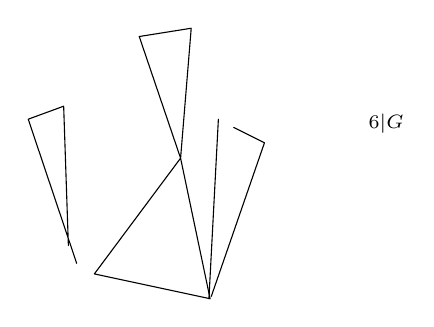
\begin{tikzpicture}[x=0.015cm,y=-0.015cm,line cap=round,line join=round]
\draw (109,1711)--(182,1613)--(207,1732)--cycle;
\draw (182,1613)--(147,1510)--(191,1503)--cycle;
\draw (206,1732)--(214,1580);
\draw (227,1587)--(253,1600)--(208,1730);
\draw (94,1702)--(53,1580)--(83,1569)--(87,1687);

\node[inner sep=1pt,font=\scriptsize] at (356,1584) {$\unsure{6|G}$};
\end{tikzpicture}}

\[
\begin{aligned}
c'_{-1,\gamma}&=6(1+c_\gamma)(1+2c_\gamma)\\
&6.\left|\begin{array}{l}1.1\\2.3\\3.5\\5.9\end{array}\right.
\end{aligned}
\]

\diagram{\(\begin{array}{c|c|c|c|c|}
{}_{\beta}\!\backslash^{\gamma}&-1&0&1&2\\\hline
-1&6=2\unsure{\cdot}3&36=2^2.3^2&90=2.3^2.5&270=2.3^3.5\\\hline
0&0&2^3.3^2\unsure{.}&2^4.3^2.5&2^6.3^3.5\\\hline
1&0&0&\begin{gathered}2^4.3^2.5\\=6!=720\end{gathered}&2^6.3^4.5\\\hline
2&0&0&0&2^7.3^{4}.5\\\hline
\end{array}\)}

% archive sheet number: 118
